\documentclass[a4paper, 10pt]{article}
\usepackage[top=1cm, bottom=1.5cm, left=1.5cm, right=1cm]{geometry}
\usepackage[utf8]{inputenc}
\usepackage{graphicx}
\usepackage[brazilian]{babel}
\usepackage[labelsep=endash, format=hang, font=small, singlelinecheck=false]{caption}

\title{CET083 - Prova prática II}
\author{Raí Bizerra}
\date{}

\begin{document}
	%Cabeçalho
	Universidade Estadual de Santa Cruz - UESC
	
	Departamento de Ciências Exatas e Tecnológicas - DCET
	
	CET083 - Probabilidade e Estatística
	
	Curso de Ciência da Computação
	
	Prof. José Cláudio Faria\\
	
	Matrículas = 201420378 201420373 201511463 \newpage	
	
	\section{AED: Apresentações tabulares e gráficas}
		\subsection{Diagrama de caixa (boxplot)}
			\subsubsection{Y1 e Y2: antes e após eliminação de possíveis outliers - sem distinção de sexo}
			%Figura 1
			\begin{figure}[!htb]
				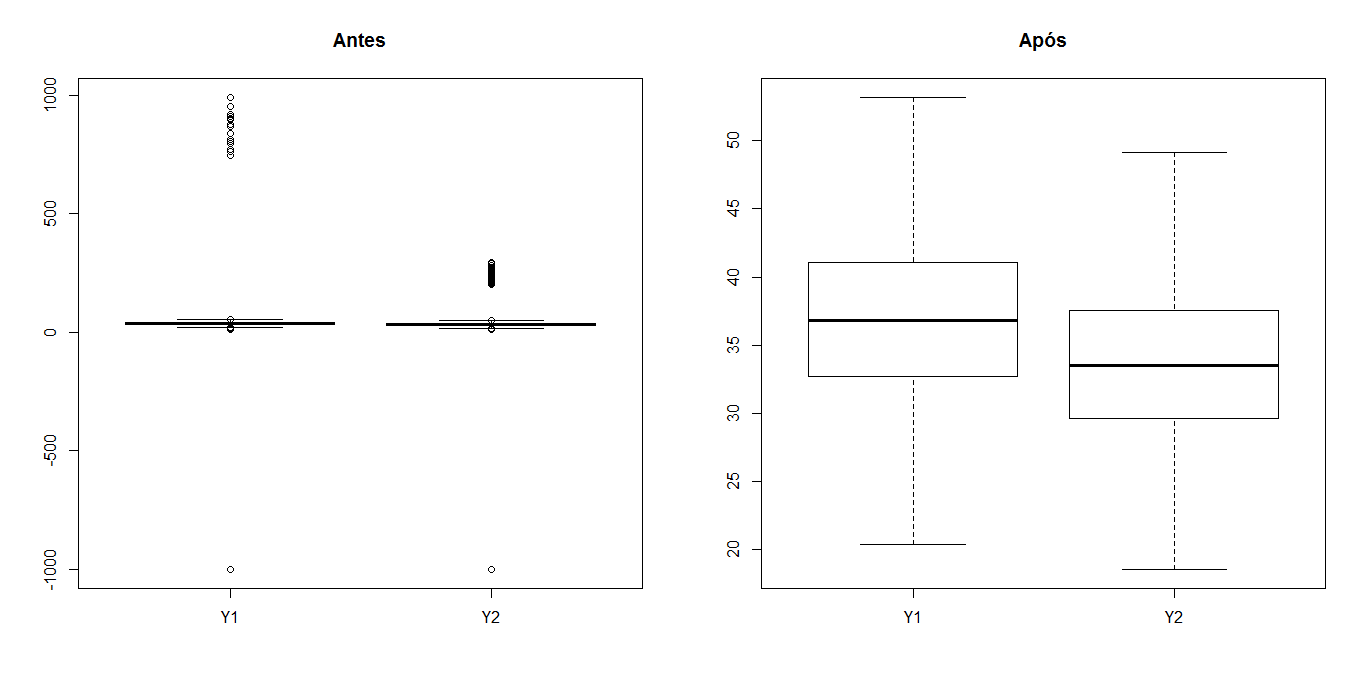
\includegraphics[width=\textwidth]{1_1_1.png}
				\caption{Diagrama de caixa de Y1 (un) e Y2 (un) antes e depois da eliminação de outliers, UESC/BA - 2017.}
			\end{figure}
		\subsubsection{Y1 e Y2: antes e após eliminação de possíveis outliers - com distinção de sexo}		
			%Figura 2
			\begin{figure}[!htb]
				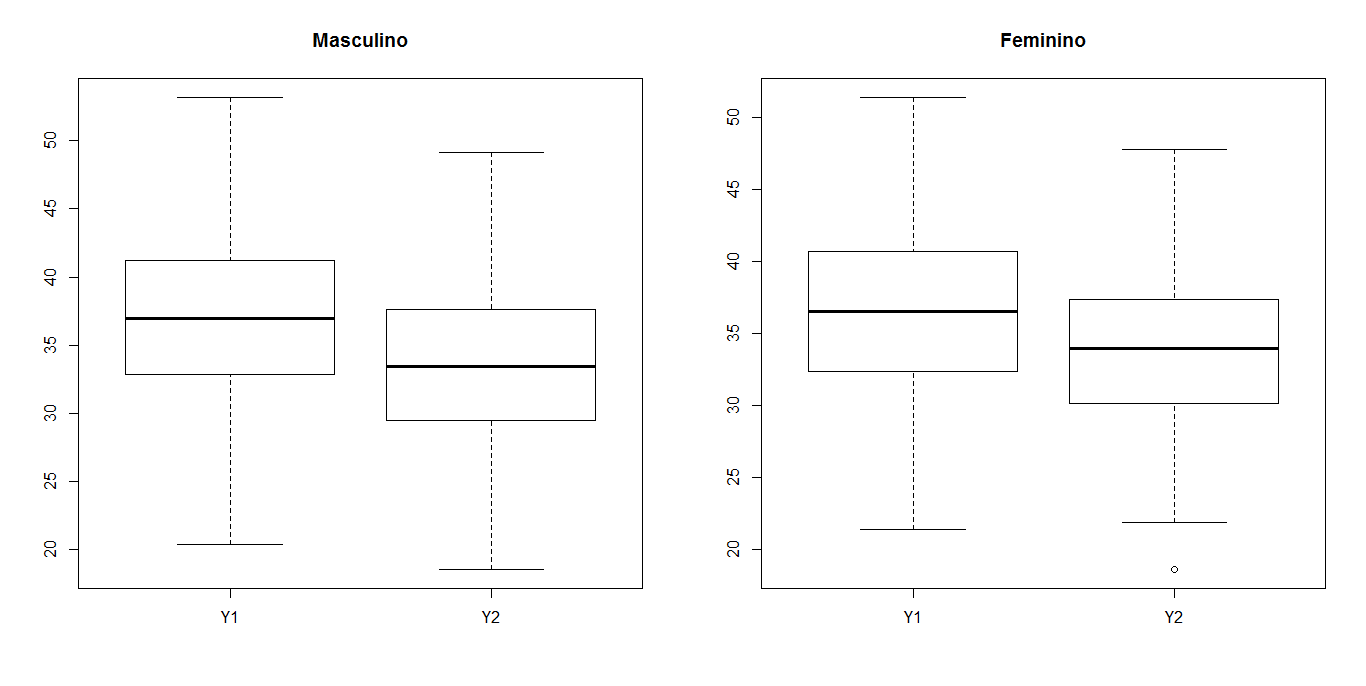
\includegraphics[width=\textwidth]{1_1_2.png}
				\caption{Diagrama de caixa de Y1 (un) e Y2 (un) (sexo masculino e feminino, respectivamente), UESC/BA - 2017.}
			\end{figure} \newpage
		\subsection{Y1}
			\subsubsection{Apresentações Tabulares}				
				\begin{table}[!htb]
					\caption{Tabela de distribuição de frequência de Y1 (un) (sexo masculino), UESC/BA - 2017}
					\begin{tabular}{rlrrr}
						\hline
						 & Class limits & f & rf(\%) & cf(\%) \\
						\hline
						 & 20.22 $\vdash$  23.01 & 8 &  0.54 & 0.54 \\
						 & 23.01 $\vdash$  25.80 & 38 & 2.56 & 3.1 \\
						 & 25.80 $\vdash$  28.59 & 69 & 4.65 & 7.75 \\
						 & 28.59 $\vdash$  31.38 & 154 & 10.38 & 18.13 \\
						 & 31.38 $\vdash$  34.17 & 238 & 16.04 & 34.16 \\
						 & 34.17 $\vdash$  36.96 & 234 & 15.77 & 49.93 \\
						 & 36.96 $\vdash$  39.75 & 260 & 17.52 & 67.45 \\
						 & 39.75 $\vdash$  42.54 & 207 & 13.95 & 81.4 \\
						 & 42.54 $\vdash$  45.33 & 139 & 9.37 & 90.77 \\
						 & 45.33 $\vdash$  48.12 & 90 & 6.06 &  96.83 \\
						 & 48.12 $\vdash$  50.91 & 35 & 2.36 &  99.19 \\
						 & 50.91 $\vdash$  53.70 & 12 & 0.81 &  100 \\
						\hline
					\end{tabular}
				\end{table}
				\begin{table}[!htb]
					\caption{Tabela de distribuição de frequência de Y1 (un) (sexo feminino), UESC/BA - 2017}
					\begin{tabular}{rlrrr}
						\hline
						 & Class limits  & f  & rf(\%)  & cf(\%) \\
						\hline
						 & 21.19 $\vdash$  24.26 & 4 & 1.08 & 1.08 \\
						 & 24.26 $\vdash$  27.33 & 14 & 3.76 & 4.84 \\
						 & 27.33 $\vdash$  30.40 & 40 & 10.75 & 15.59 \\
						 & 30.40 $\vdash$  33.47 & 61 & 16.4 & 31.99 \\
						 & 33.47 $\vdash$  36.54 & 68 & 18.28 & 50.27 \\
						 & 36.54 $\vdash$  39.61 & 69 & 18.55 & 68.82 \\
						 & 39.61 $\vdash$  42.68 & 67 & 18.01 & 86.83 \\
						 & 42.68 $\vdash$  45.75 & 27 & 7.26 & 94.09 \\
						 & 45.75 $\vdash$  48.82 & 16 & 4.3 & 98.39 \\
						 & 48.82 $\vdash$  51.89 & 6 & 1.61 & 100 \\
						\hline
					\end{tabular}
				\end{table} \newpage
			\subsubsection{Histograma e polígono de frequência acumulada}
				%Figura 3
				\begin{figure}[!htb]
					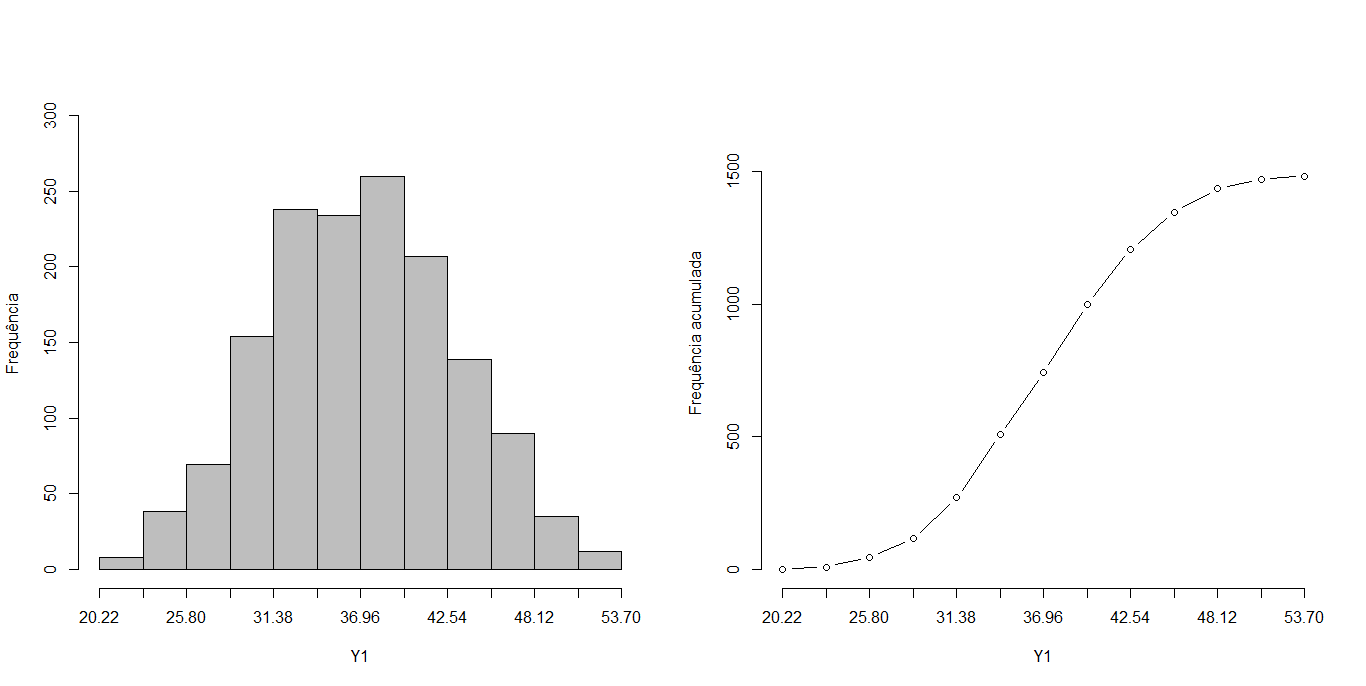
\includegraphics[width=\textwidth]{1_2_2m.png}
					\caption{Histograma e polígono de frequência acumulada de Y1 (un) (sexo masculino), UESC/BA - 2017.}
				\end{figure}
				% Figura 4
				\begin{figure}[!htb]
					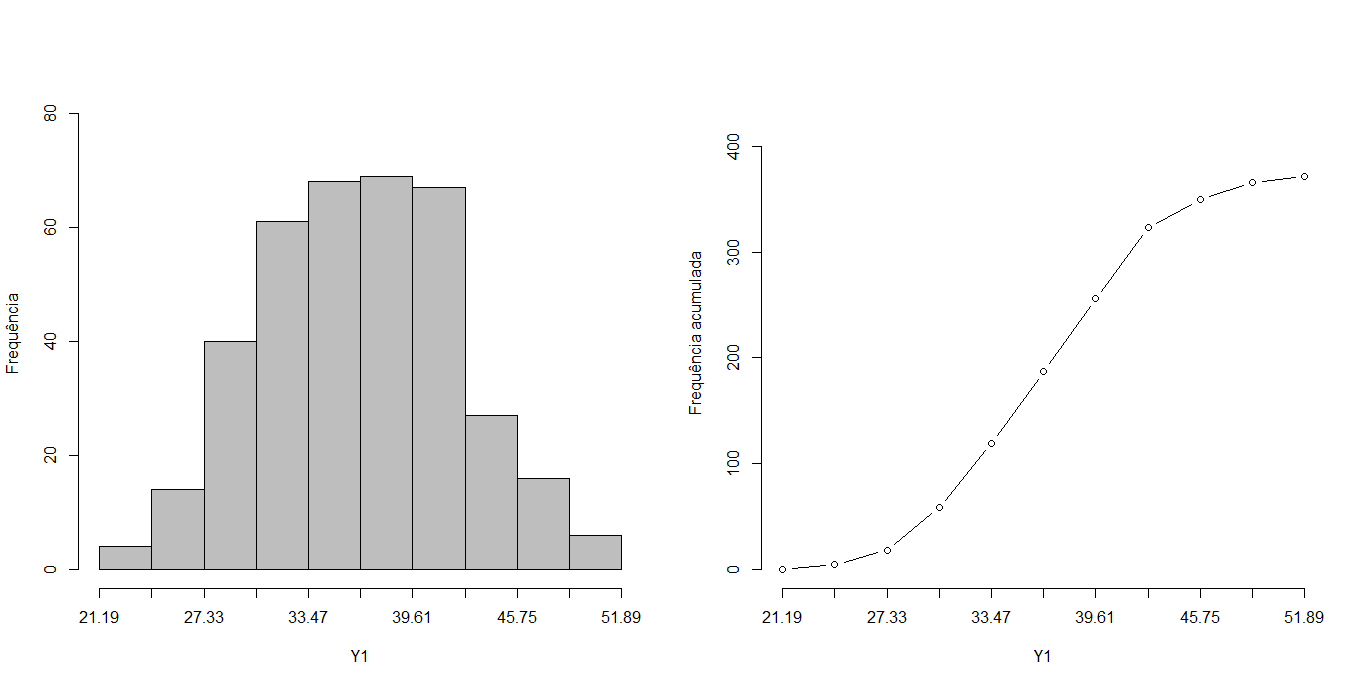
\includegraphics[width=\textwidth]{1_2_2f.png}
					\caption{Histograma e polígono de frequência acumulada de Y1 (un) (sexo feminino), UESC/BA - 2017.}
				\end{figure} \newpage
	\section{AED: Medidas estatísticas básicas}
		\subsection{Tendência Central}
			\begin{table}[!htb]
				\caption{Medidas de tendência central (sexo masculino), UESC/BA - 2017}
				\begin{tabular}{crrr}
					\hline
					& n & m & md \\
					\hline
					Y1 & 1484 & 36.98 & 36.97 \\
					Y2 & 1484 & 33.58 & 33.52 \\
					\hline
				\end{tabular}
			\end{table}
			\begin{table}[!htb]
				\caption{Medidas de tendência central (sexo feminino), UESC/BA - 2017}
				\begin{tabular}{crrr}
					\hline
					& n & m & md \\
					\hline
					Y1 & 372 & 36.48 & 36.49 \\
					Y2 & 372 & 33.78 & 33.8 \\
					\hline
				\end{tabular}
			\end{table}
		\subsection{Posição}
			\begin{table}[!htb]
				\caption{Quartis dos usuários(sexo masculino), UESC/BA - 2017}
				\begin{tabular}{crrr}
					\hline
					& 25\% & 50\% & 75\% \\
					\hline
					Y1 & 32.86 & 36.97 & 41.21 \\
					Y2 & 29.50 & 33.42 & 37.60 \\
					\hline
				\end{tabular}
			\end{table}
			\begin{table}[!htb]
				\caption{Quartis dos usuários(sexo feminino), UESC/BA - 2017}
				\begin{tabular}{crrr}
					\hline
					& 25\% & 50\% & 75\% \\
					\hline
					Y1 & 32.36 & 36.48 & 40.68 \\
					Y2 & 30.13 & 33.97 & 37.32 \\
					\hline
				\end{tabular}
			\end{table}
			\begin{table}[!htb]
				\caption{Decis dos usuários(sexo masculino), UESC/BA - 2017}
				\begin{tabular}{crrrrrrrrr}
					\hline
					& 10\% & 20\% & 30\% & 40\% & 50\% & 60\% & 70\% & 80\% & 90\% \\
					\hline
					Y1 & 29.44 & 31.69 & 33.59 & 35.39 & 36.97 & 38.56 & 40.24 & 42.23 & 45.14 \\
					Y2 & 26.13 & 28.64 & 30.36 & 32.05 & 33.41 & 34.91 & 36.67 & 38.62 & 41.05 \\
					\hline
				\end{tabular}
			\end{table}
			\begin{table}[!htb]
				\caption{Decis dos usuários(sexo masculino), UESC/BA - 2017}
				\begin{tabular}{crrrrrrrrr}
					\hline
					& 10\% & 20\% & 30\% & 40\% & 50\% & 60\% & 70\% & 80\% & 90\% \\
					\hline
					Y1 & 29.37 & 31.51 & 33.06 & 35.21 & 36.48 & 37.98 & 39.83 & 41.59 & 44.00\\
					Y2 & 26.82 & 29.43 & 31.07 & 32.38 & 33.97 & 35.27 & 36.43 & 38.34 & 41.16\\
					\hline
				\end{tabular}
			\end{table}
		\subsection{Dispersão}
			\begin{table}[!htb]
				\caption{Dispersão  dos usuários(sexo masculino), UESC/BA - 2017}
				\begin{tabular}{crrrr}
					\hline
					& A.T & Variância & D.Padrão & C.V \\
					\hline
					Y1 & 32.75 & 35.75 & 5.98 & 16.15 \\
					Y2 & 30.54 & 32.01 & 5.66 & 16.87 \\
					\hline
				\end{tabular}
			\end{table}
			\begin{table}[!htb]
				\caption{Dispersão  dos usuários(sexo masculino), UESC/BA - 2017}
				\begin{tabular}{crrrr}
					\hline
					& A.T & Variância & D.Padrão & C.V \\
					\hline
					Y1 & 29.98 & 33.08 & 5.75 & 15.74 \\
					Y2 & 29.16 & 28.48 & 5.34 & 15.75 \\
					\hline
				\end{tabular}
			\end{table}
	\section{AED: Medidas estatísticas de associação e regressão linear}
		\subsection{Associação}
			\subsubsection{Estimativas: covariância e correlação linear simples.}
				\begin{table}[!htb]
					\caption{Matriz de variâncias e covariâncias (sexo masculino), UESC/BA – 2017}
					\begin{tabular}{ccc}
						\hline
						& Y1 & Y2  \\
						\hline
						Y1 & 35.75 & 32.31 \\
						Y2 & 32.31 & 32.01 \\
						\hline
					\end{tabular}
				\end{table}
				\begin{table}[!htb]
					\caption{Matriz de variâncias e covariâncias (sexo feminino), UESC/BA – 2017}
					\begin{tabular}{ccc}
						\hline
						& Y1 & Y2  \\
						\hline
						Y1 & 33.08 & -23.95 \\
						Y2 & -23.95 & 28.48 \\
						\hline
					\end{tabular}
				\end{table}
				\begin{table}[!htb]
					\caption{Matriz de correlações lineares simples (sexo masculino), UESC/BA – 2017}
					\begin{tabular}{ccc}
						\hline
						& Y1 & Y2  \\
						\hline
						Y1 & 1.00 & 0.96 \\
						Y2 & 0.96 & 1.00 \\
						\hline
					\end{tabular}
				\end{table}
				\begin{table}[!htb]
					\caption{Matriz de correlações lineares simples (sexo feminino), UESC/BA – 2017}
					\begin{tabular}{ccc}
						\hline
						& Y1 & Y2  \\
						\hline
						Y1 & 1.00 & -0.78 \\
						Y2 & -0.78 & 1.00 \\
						\hline
					\end{tabular}
				\end{table}
			\subsubsection{Diagrama de dispersão dos dados}
				% Figura 4
				\begin{figure}[!htb]
					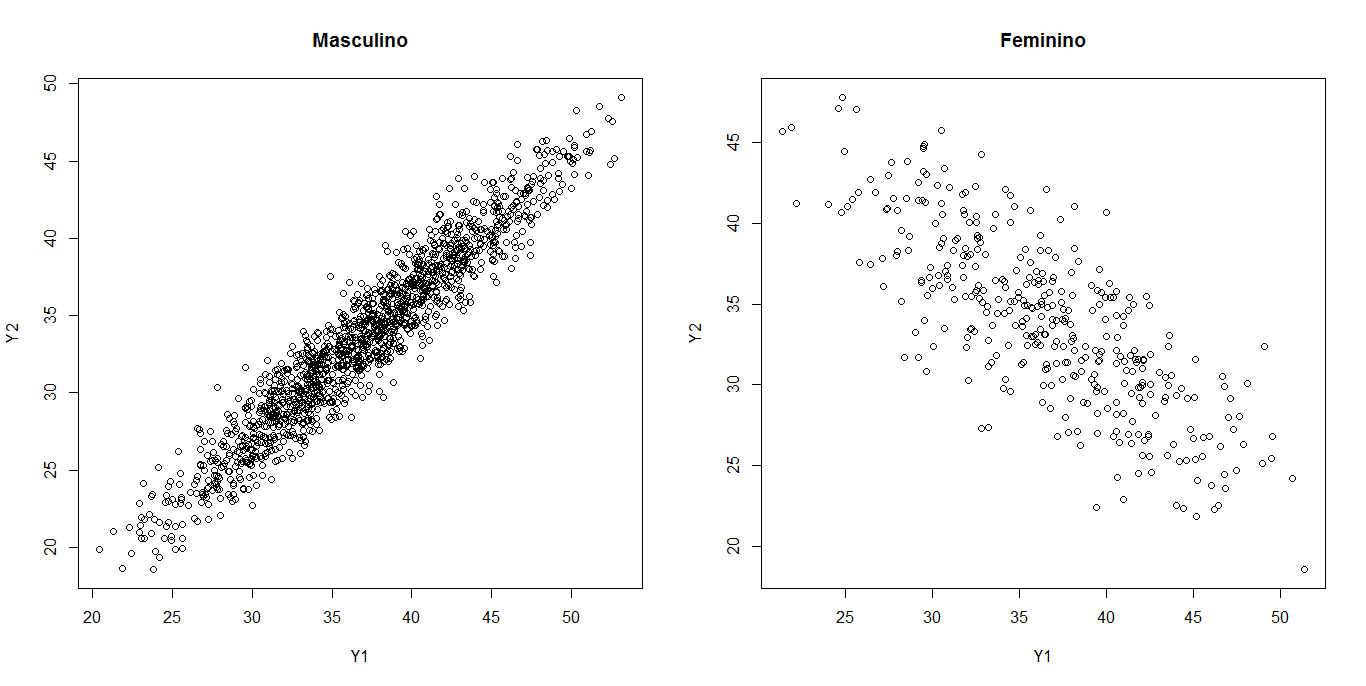
\includegraphics[width=\textwidth]{3_1_2.png}
					\caption{Diagrama de dispersão de Y1 (un) e Y2 (un) (sexo masculino e feminino, respectivamente), UESC/BA - 2017.}
				\end{figure}
			\subsubsection{Comparação de estudos semelhantes}
				Para comparar associações entre as variáveis de ambos os estudos, seria recomendada a medida de \textbf{Correlação}, porque esta não é influenciada por unidades de medida.
		\subsection{Regressão linear}
			\subsubsection{Ajustamento}
				\begin{table}[!htb]
					\caption{Estimativa dos parâmetros polinômio grau I, UESC/BA - 2017}
					\begin{tabular}{rrrrr}
						\hline
						& Estimate & Std. Error & t value & Pr($>|$t$|$)  \\
						\hline
						(Intercept) & 3.33 & 0.79 & 4.21 & 0.00 \\
								X &	1.11 & 0.13 & 8.35 & 0.00 \\
						\hline
					\end{tabular}
				\end{table}
				\begin{table}[!htb]
					\caption{Estimativa dos parâmetros polinômio grau II, UESC/BA - 2017}
					\begin{tabular}{rrrrr}
						\hline
						& Estimate & Std. Error & t value & Pr($>|$t$|$) \\ 
						\hline
						(Intercept) & 1.81 & 0.73 & 2.47 & 0.04 \\ 
						X & 2.14 & 0.34 & 6.27 & 0.00 \\ 
						I(X\verb|^|2) & -0.10 & 0.03 & -3.12 & 0.01 \\ 
						\hline
					\end{tabular}
				\end{table}
			\subsubsection{Diagrama de dispersão}
				% Figura 5
				\begin{figure}[!htb]
				\centering
					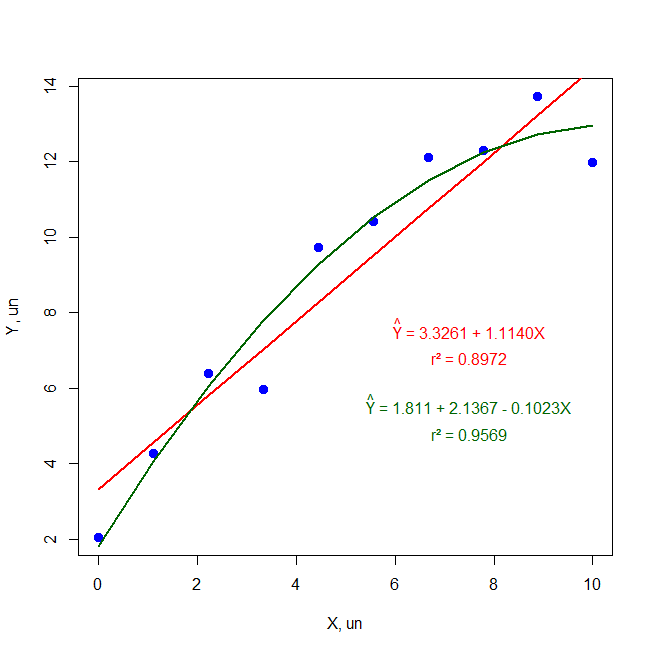
\includegraphics[scale=0.5]{3_2_2.png}
					\caption{Diagrama de dispersão dos dados, modelos ajustados e respectivos r$^{2}$.}
				\end{figure}
			\subsubsection{Opção entre os modelos}	
	\section{Contextualização}
\end{document}
